\documentclass{article}

\usepackage[paperwidth=8.5in,paperheight=11in,left=1.4in,
right=1in,top=1.3in, bottom=1.4in]{geometry}
\usepackage{sectsty, tikz, color, pgfplots}
\usetikzlibrary{shapes,arrows}
\usetikzlibrary{fit}
\makeatletter
\tikzset{
  fn/.style={
    inner sep=0pt,
    fill=none,
    draw=none,
    reset transform,
    fit={(\pgf@pathminx,\pgf@pathminy) (\pgf@pathmaxx,\pgf@pathmaxy)},
  },
  reset transform/.code={\pgftransformreset}
}
\makeatother

    \usetikzlibrary{patterns}
    \tikzset{%
        dotsfill/.style={draw,pattern=dots},
    }

\pgfdeclarepatternformonly[\StripesSize]{MyStripes}{\pgfqpoint{-1pt}{-1pt}}{\pgfqpoint{4pt}{4pt}}{\pgfqpoint{\StripesSize}{\StripesSize}}%
{
  \pgfsetlinewidth{0.3pt}
  \pgfpathmoveto{\pgfqpoint{0pt}{0pt}}
  \pgfpathlineto{\pgfqpoint{3.1pt}{3.1pt}}
  \pgfusepath{stroke}
}

\newdimen\StripesSize
\tikzset{
    StripesSize/.code={\StripesSize=#1},
    StripesSize=3pt
}

\begin{document}
\pagestyle{empty}
\begin{figure}
  \centering
    \noindent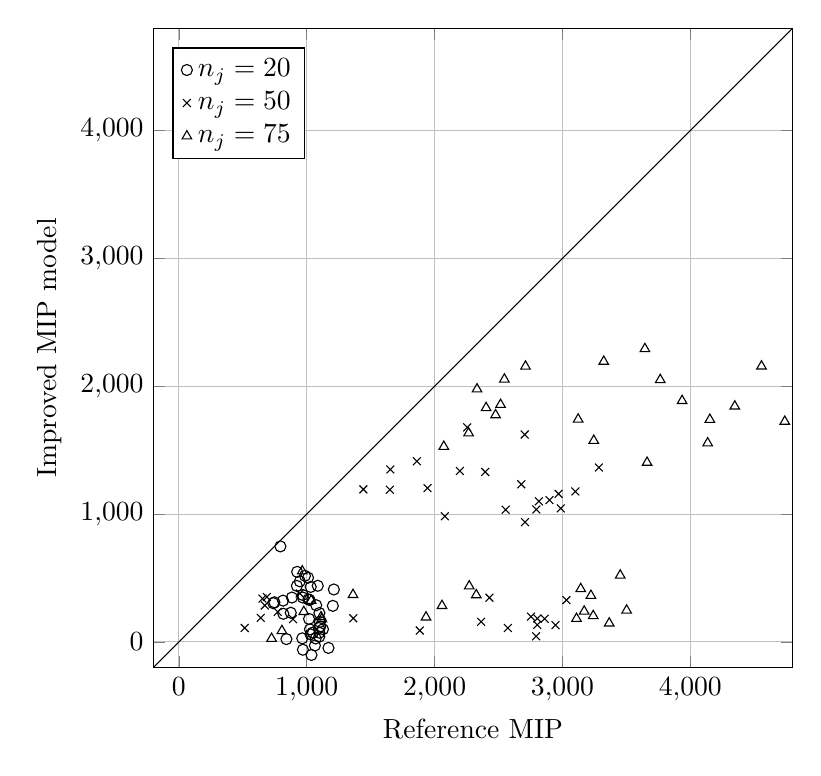
\begin{tikzpicture}

  \begin{axis}[width=0.8\textwidth, 
  height=0.8\textwidth,xmin=-200, xmax=4800, ymin=-200,
  ymax=4800,
  y tick label style={
        /pgf/number format/.cd,
            fixed,
            fixed zerofill,
            precision=0,
        /tikz/.cd
    }, 
     x tick label style={
        /pgf/number format/.cd,
            fixed,
            fixed zerofill,
            precision=0,
        /tikz/.cd
    }, grid,
    log ticks with fixed point, 
    legend pos = north west,
    xlabel=Reference MIP, ylabel=Improved MIP
    model]
\addplot[color=black, mark=o,only marks] coordinates {
(925, 548)
(1204, 282)
(817, 220)
(1170, -47)
(1010, 502)
(815, 323)
(1127, 99)
(970, -61)
(1013, 333)
(1031, 430)
(1070, 27)
(1037, -102)
(738, 303)
(1022, 328)
(1018, 180)
(1048, 73)
(1212, 410)
(884, 347)
(1025, 98)
(1098, 41)
(969, 367)
(747, 310)
(1099, 72)
(1048, 72)
(1099, 226)
(794, 747)
(1074, 287)
(1106, 121)
(965, 28)
(946, 474)
(1086, 439)
(1103, 157)
(1064, -28)
(986, 517)
(923, 438)
(1030, 59)
(841, 22)
(970, 347)
(875, 228)
(1095, 109)

};
\addlegendentry{$n_j = 20$}

\addplot[color=black, mark=x,only marks] coordinates {
(1654, 1349)
(2707, 937)
(2861, 181)
(2804, 183)
(2705, 1622)
(3101, 1177)
(1364, 185)
(2573, 109)
(1945, 1203)
(2970, 1158)
(672, 285)
(515, 109)
(2816, 1100)
(1861, 1413)
(640, 188)
(688, 351)
(2080, 983)
(2556, 1034)
(945, 379)
(773, 235)
(2678, 1233)
(1650, 1190)
(2754, 198)
(2794, 44)
(2255, 1678)
(3285, 1364)
(893, 178)
(2946, 131)
(2396, 1329)
(2899, 1109)
(654, 339)
(3031, 327)
(1443, 1193)
(2987, 1044)
(2429, 346)
(1884, 89)
(2198, 1337)
(2796, 1036)
(2364, 157)
(2803, 133)

};
\addlegendentry{$n_j = 50$}
\addplot[color=black, mark=triangle,only marks] coordinates {
(3936, 1886)
(3123, 1741)
(1933, 193.0000)
(3143, 415)
(3245, 1575)
(4739, 1724)
(3170, 239)
(806, 87)
(3323, 2193)
(2266, 1633)
(977, 236)
(965, 554)
(2546, 2054)
(2516, 1856)
(3241, 204)
(3223, 362)
(3765, 2050)
(2072, 1528)
(1112, 195)
(1035, 323)
(4557, 2156)
(3645, 2292)
(1118, 179)
(3110, 182)
(2403, 1831)
(4348, 1843)
(3366, 146)
(2271, 436)
(2477, 1775)
(4153, 1739)
(3452, 521)
(3502, 247)
(2711, 2155)
(3662, 1403)
(1362, 369)
(725, 26)
(2332, 1977)
(4136, 1555)
(2326, 367)
(2058, 283)
};
\addlegendentry{$n_j=75$}


\addplot[draw=black] coordinates {(-200,-200) (4800, 4800)};

  \end{axis}
\end{tikzpicture}
   \vspace{0.73em}
\end{figure}
\end{document}
